\chapter{Grundlagen\label{chap2:Zweites-Kapitel}}

Um eine Konzeption und eine prototypische Umsetzung einer Search Engine in \gls{mcc} zu ermöglichen wird in folgendem Kapitel auf die architekturellen Hintergründe von \gls{mcc} eingegangen. Hierfür werden zu Beginn allgemein gültige Architektur-Prinzipien erläutert, welche auch bei der Integration einer Search Engine berücksichtigt werden müssen und somit bei der Auswahl eines geeigneten Konzeptes von Bedeutung sind.

Aufbauend auf den Architektur-Prinzipien wird die verwendete Microservice-Architektur erläutert, wobei neben einer allgemeinen Einführung in die Architektur auch auf die Kommunikation von Microservices untereinander eingegangen wird. Um mögliche Fehlkonzeptionen zu vermeiden, werden häufig auftretende Anti-Pattern aufgezeigt, welche unter Umständen zu monolithischen Seiteneffekten führen könnten.

\section{Software-Architekturen\label{sec2.1:Unterpunkt-1}}

\begin{quote}
    Die Software-Architektur eines Systems ist die Menge von Strukturen, die benötigt werden, um Entscheidungen über das System zu treffen, welche die Software-Elemente, die Relationen zwischen ihnen und die Eigenschaften von beiden betreffen. \textasciitilde{} Len Bass \cite{Bass.2013}
\end{quote}

Wie aus der Definition von Len Bass zu entnehmen ist, beschreibt eine Software-Architektur die Eigenschaften und Beziehungen von Software-Bausteinen zueinander \cite{Bass.2013}. Ein Software-Baustein wird hierbei als eine Teil-Komponente der gesamten Software betrachtet und wird bei der Erstellung einer Architektur als elementarer Bestandteil angesehen. Dabei wird ein Software-Baustein nicht näher spezifiziert, sondern als Komponente betrachtet, dessen konkrete Implementierung für die Architektur nicht von Bedeutung ist. Der Fokus einer Software-Architektur liegt auf den Schnittstellen der Software-Bausteine, über welche die Bausteine miteinander kommunizieren können.

\subsection{Architektur-Prinzipien\label{subsec2.1.1:Unterunterpunkt-1}}

Für das Erstellen einer guten Software-Architektur wurden von Vogel \cite{Vogel.2009} einige Grundprinzipien definiert. Diese Prinzipien sollten bei der Erstellung einer Software-Architektur beachtet werden: \cite{Vogel.2009}

\begin{description}
    \item[Lose Kopplung:]\hfill \\
    Der Kern einer Software-Architektur besteht aus der Beschreibung der Bausteine eines Software-Systems und deren Interaktionen zueinander. Unter dem Begriff Kopplung versteht man hierbei die Beziehung unter den Bausteinen einer Software-Architektur. Eine Kopplung charakterisiert demnach die Interaktionen der Bausteine.

    Eine starke Kopplung von Systembausteinen hat zur Folge, dass beim Verstehen und Ändern eines Bausteines auch zwingend weitere Bausteine verstanden und geändert werden müssen. Um jenes Problem zu umgehen, besagt das Prinzip der losen Kopplung, dass die Kopplung zwischen Systembausteinen möglichst niedrig gehalten werden sollen.

    Um eine lose Kopplung in einer Architektur zu erreichen, ist die Einführung von Schnittstellenabstraktionen ein wichtiger Aspekt. Dabei werden die Implementierungsinformationen hinter den Schnittstellen verborgen. Durch die Begrenzung von Schnittstellenelementen und der Häufigkeit des Austauschs der Schnittstellenelemente kann eine Kopplung von Systembausteinen kontrollierbar gemacht werden.

    \item[Hohe Kohäsion:]\hfill \\
    Im Gegensatz zur Kopplung, in welcher die Beziehungen zwischen Systembausteinen gemeint ist, versteht man unter dem Begriff Kohäsion die Abhängigkeiten innerhalb eines Systembausteins.

    Beim Prinzip der hohen Kohäsion ist das Ziel die Abhängigkeiten innerhalb eines Systembausteins möglichst hoch zu gestalten. Wie bei der losen Kopplung geht es auch hier um die lokale Änderbarkeit und Verstehbarkeit von Systembausteinen.
    
    Wie in \autoref{fig:kopplung_and_kohaesion} zu erkenne stehen Kopplung und Kohäsion normalerweise miteinander in einer Wechselbeziehung. Hierbei gilt, dass je höher die Kohäsion individueller Bausteine einer Architektur ist, desto geringer ist die Kopplung zwischen den Bausteinen. Schematisch ist dieser Zusammenhang in \autoref{fig:kopplung_and_kohaesion} abgebildet, worin zu erkennen ist, das eine Gesamtstruktur mit einer hohen Kohäsion und einer losen Kopplung (rechte Seite) eine höhere Übersichtlichkeit besitzt.

    \begin{figure}[H]
        \centering
        \includegraphics[width=0.7\linewidth]{images/Kopplung_und_Kohäsion.png}
        \caption{Zusammenspiel von loser Kopplung und hoher Kohäsion - \cite{Vogel.2009}}
        \label{fig:kopplung_and_kohaesion}
    \end{figure}

    \item[Entwurf für Veränderung:]\hfill \\
    Durch den stetigen Wandel von Software-Systemen in Form von Anforderungen und Technologien, ist es von Vorteil solche Änderungen bereits in der Phase der architekturellen Konzeption zu berücksichtigen. Das Prinzip des Entwurfs für Veränderung (englisch: Design for Change) sieht nun vor, dass man vorhersehbare Änderungen architektonisch vorausplant. Dabei sollte man versuchen, die Architektur so zu entwerfen, dass man leicht mit den wahrscheinlichen Änderungen eines Software-Systems umgehen kann.

    \item[Separation of Concerns:]\hfill \\
    Abgeleitet von dem römischen Prinzip \glqq Teile und herrsche\grqq{} wird beim Prinzip Separation of Concerns ausgesagt, dass ein Software-System in individuelle Systembausteine zerlegt werden soll.

    Separation of Concerns unterstützt hierbei die Modularisierung eines Software-Systems. Es geht darum Teile eines Software-Systems zu identifizieren, welche für bestimmte Angelegenheiten, Aspekte und Aufgaben verantwortlich sind. Jene Teile werden dann als eigene Systembausteine gekapselt. Eine Zerteilung des Gesamtsystems in relativ unabhängige Einzelteile ermöglicht zudem noch die Verteilung von Verantwortlichkeiten für verschiedene Systembausteine und auch das parallele Arbeiten an dem Software-System durch mehrere Entwickler wird dadurch ermöglicht.

    Durch das Aufteilen des Software-Systems in relativ unabhängige Systembausteine werden auch die Prinzipien lose Kopplung und hohe Kohäsion begünstigt.

    \item[Information Hiding:]\hfill \\
    Das Prinzip Information Hiding sagt aus, dass man einem Klienten nur die für die Bearbeitung eines Problems notwendigen Informationen zeigen soll. Dies erleichtert die Gliederung und das Verständnis von komplexen Software-Systemen. Die restlichen Informationen sollen nach außen hin verborgen bleiben. Ermöglicht wird solch ein geheim halten von Informationen durch die Bereitstellung von definierten Schnittstellen, über welche nur bestimmte Informationen zu erreichen sind.

    \item[Abstraktion:]\hfill \\
    Als übergeordnetes Prinzip dient eine Abstraktion dazu, ein komplexes System verständlicher zu machen. Dazu werden wichtige Aspekte identifiziert und unwichtige Details vernachlässigt. Im Bereich der Software-Architektur gilt die Schnittstellenabstraktion als Teilprinzip der Abstraktion. Hierbei liegen die Schnittstellen im Fokus, welche für das Zustandekommen und die Qualität von Beziehungen verantwortlich sind.

    Solch eine Schnittstellenabstraktion in einem Software-System ist eng verbunden mit dem Prinzip der losen Kopplung und dem Information Hiding. Ein Aspekt für den starken Zusammenhang zwischen der Abstraktion und dem Information Hiding ist die Portabilität von Software-Systemen. So sollte eine Architektur oder ihre Systembausteine auch in anderen Umgebungen verwendbar sein. Um solch eine Plattformunabhängigkeit sicherzustellen, werden Abstraktionen verwendet, die ein Information Hiding der Platform-Details leisten.

    \item[Modularität:]\hfill \\
    Das Modularitätsprinzip, welches bereits auch in den Beschreibungen der anderen Prinzipien vorkam, definiert die Aufteilung eines Systems in klar definierte Bausteine mit abgegrenzten funktionalen Verantwortlichkeiten. Die Modularität ist dabei eine Kombination aus den Prinzipien Abstraktion, Separation of Concerns und Information Hiding, welche bei der Umsetzung der Prinzipien der losen Kopplung und der hohen Kohäsion kombiniert werden.

\end{description}

Auch für die spätere Konzeption einer Search Engine in einer Microservice-Architektur werden die eingeführten Prinzipien als Grundlage dienen.

\subsection{Monolithische und verteilte Architekturen\label{subsec2.1.2:Unterunterpunkt-2}}

Bei der Neugestaltung von E-MES wird von einer monolithischen 3-Schichten-Architektur auf eine verteilte Microservice-Architektur gewechselt.

Dabei besaß die ehemalige E-MES Architektur eine monolithische Struktur. In einer solchen monolithische Architektur wird die gesamte Architektur in nur einem Systembaustein zusammengefasst. Dadurch erfolgt keine explizite Gliederung in Teilsysteme und Architektur-Prinzipien, wie lose Kopplung und Separation of Concerns sind nur schwer umsetzbar \cite{Vogel.2009}. Zu finden sind monolithische Architekturen oftmals in Altsystemen, welche oft über Jahrzehnte gewachsen sind. Aufgrund der mangelnden Modularisierung steigt die Kompliziertheit des Systems und eine Wartung und Anpassung des Quellcodes wird erschwert \cite{Prof.Dr.AndreasFink.2012b}. Ein weiterer Nachteil der mangelnden Modularisierung ist die kaum mögliche nebenläufige Ausführung von Teilen des Systems auf verschiedenen Rechnern \cite{Prof.Dr.AndreasFink.2012b}. Somit kann eine horizontale Skalierung nicht ermöglicht werden und eine effiziente, lastverteilende Programmausführung ist nicht gegeben.

Die Architektur von MCC wird eine verteilte Struktur aufweisen. Hierbei werden Teile des Gesamtsystems in unterschiedliche Systembausteine aufgeteilt. Eine Modularisierung der Software ist dadurch möglich und Architekturen-Prinzipien, wie lose Kopplung und Separation of Concerns sind umsetzbar \cite{Vogel.2009}. Durch die strikte Aufteilung der Geschäftslogik kann auch die Komplexität aufgeteilt werden. Somit können die einzelnen Systembausteine mit wenig Aufwand angepasst oder erweitert werden. Durch die Modularisierung von verteilten Architektur kann die Ausführung bestimmter Aufgaben auf redundanter Hardware nebenläufig erfolgen \cite{Prof.Dr.AndreasFink.2012}. Durch jene horizontale Skalierung kann eine effiziente und lastverteilende Programmausführung erfolgen, welche auch zur Ausfallsicherheit des Gesamtsystems beiträgt \cite{Prof.Dr.AndreasFink.2012}.

\section{Microservice-Architektur\label{sec2.2:Unterpunkt-2}}

Als eine Architektur mit einer verteilten Struktur, wird die Software bei der Neugestaltung des \gls{mes} der Firma Enisco, auf einer Microservice-Architektur aufgebaut.

Die Kernelemente dieser Architektur sind die Microservices, welche der Modularisierung der Software dienen. Somit ist eine Aufteilung des Gesamtsystems in verschiedene Systembausteine möglich. Ein Systembaustein stellt dabei jeweils eine Funktionalität des Gesamtsystems dar. Im Gegensatz zu einer monolithischen Architektur läuft das Gesamtsystem nicht innerhalb eines Prozesses, sondern auf verschiedenen Prozessen. Dabei wird jedem Systembaustein ein eigener Prozess zugeordnet. Jene Prozesse können nun nahezu beliebig auf verschiedene Rechner verteilt und durch Replizierung ausfallsicher gemacht werden. \cite{GaryCalcott.2018}

Neben den Vorteilen der horizontalen Skalierung, ergeben sich aus der Aufteilung des Gesamtsystems in unterschiedliche Systembausteine auch Auswirkungen auf die Entwicklungsorganisation. So wird beim Umgang mit Microservices nach der Unix-Philosophie von Ken Thompson \glqq Do one thing and do ot well\grqq{} \cite{IONOSSE.2021} gearbeitet. Durch die Modularität von Microservices untereinander können die Microservices von unterschiedlichen Entwicklerteams unabhängig voneinander entwickelt werden. Durch die Abstraktion der Microservices, können diese mit unterschiedlichen Technologien und Programmiersprachen implementiert werden. Auch der Datenhaushalt kann von jedem Microservice separat verwaltet werden. Zudem wird die Einarbeitung eines Entwicklers in die Codebasis reduziert, da durch die Aufteilung weniger Code verstanden werden muss.

Die Microservice-Architektur berücksichtigt die Architektur-Prinzipien Separation of Concerns, Information Hiding und Modularität und gewährleisten somit eine lose Kopplung zwischen den Microservices. Innerhalb der Microservices entsteht dadurch eine hohe Kohäsion.

Da die jeweiligen Microservices repliziert auf verschiedenen Rechnern laufen können, ist die Kommunikation zwischen den Microservices schwieriger als bei einem monolithischen System. Auf die Kommunikation zwischen Microservices wird in \autoref{subsec2.2.1:Unterunterpunkt-1} näher eingegangen.

Eine Herausforderung bei der Entwicklung einer Microservice-Architektur ist die Vermeidung von Abhängigkeiten, welche eine lose Kopplung der Microservices verhindern. Um solche monolithischen Seiteneffekten zu vermeiden, werden in \autoref{subsec2.2.2:Unterunterpunkt-2} die häufigsten Microservice-Antipattern aufgezeigt.

\subsection{Kommunikation zwischen Microservices\label{subsec2.2.1:Unterunterpunkt-1}}

Auch wenn das Ziel einer Microservice-Architektur ist, dass einzelne Funktionalitäten des Gesamtsystems in getrennte Microservices gekapselt werden, müssen jene miteinander kommunizieren. Aufgrund der Modularität können die Microservices horizontal skaliert werden und auf verschiedenen Rechnern betrieben werden. Dies erhöht die Komplexität bei der Kommunikation der Microservices untereinander. \cite{MichaelSchwab.2019}

Bei der Wahl der Kommunikation zwischen Microservices kann zwischen einer synchronen und asynchronen Kommunikation entschieden werden.

\subsubsection*{Synchrone Kommunikation}

Bei der synchronen Kommunikation handelt es sich um eine eins-zu-eins Kommunikation, bei der eine Anfrage geschickt und auf eine Antwort gewartet wird. Klassischerweise erfolgt die Kommunikation über HTTP mit einer REST-Schnittstelle. \gls{rest} ist hierbei eine Spezifikation, wie eine über HTTP kommunizierende API konzipiert werden soll \cite{MichaelSchwab.2019}. Eine solche API sollte demnach vordefinierte HTTP-Methoden implementiert haben. Unter anderem sind das Methoden wie GET, POST, PUT und DELETE. Bei einer GET-Anfrage werden hierbei Ressourcen angefragt. Möchte man einen neuen Datensatz übermitteln wird die POST-Methode verwendet und wenn man einen bestehenden Datensatz ändern möchte, verwendet man die PUT-Methode. Mit der DELETE-Methode kann man einen expliziten Datensatz löschen. Jeder Datensatz bekommt hierbei einen eigenen Endpunkt und die jeweiligen Anfragen können mit URL-Parametern und Query-Parametern spezifiziert werden. Das Standard-Datenformat bei REST ist JSON.

\label{service_discovery}Bei der Kommunikation von zwei Microservices über die jeweiligen REST-Schnittstellen, muss die Adresse des anderen Microservice bekannt sein. Durch die Verteilung der Microservices auf unterschiedliche Rechner in Folge einer horizontalen Skalierung kann es während dem Betrieb vorkommen, dass einzelne Microservices auf zum Beispiel Rechner A gestoppt und auf Rechner B wieder gestartet werden. Dadurch ändern sich auch die Adressen der Microservices. Da die Verwaltung der Adressen ab einer Vielzahl an Microservices nicht mehr trivial ist, wird in einer Microservice-Architektur eine sogenannte Service-Discovery eingesetzt. Die Service-Discovery ist eine Software, bei der sich alle neuen Microservice registrieren. Bei einem REST-Aufruf wird dann zuerst eine Liste mit allen verfügbaren Adressen abgerufen.

Wie in \autoref{fig:service_discovery} abgebildet ist, wird bei einer Anfrage eines Services, jene Anfrage zunächst an einen Router-Service geleitet. Nach dem Abfragen der Adresse mithilfe der Service-Discovery wird gezielt der entsprechende Service beziehungsweise dessen Instanz mit einer REST-Anfrage angesprochen.

\begin{figure}[H]
    \centering
    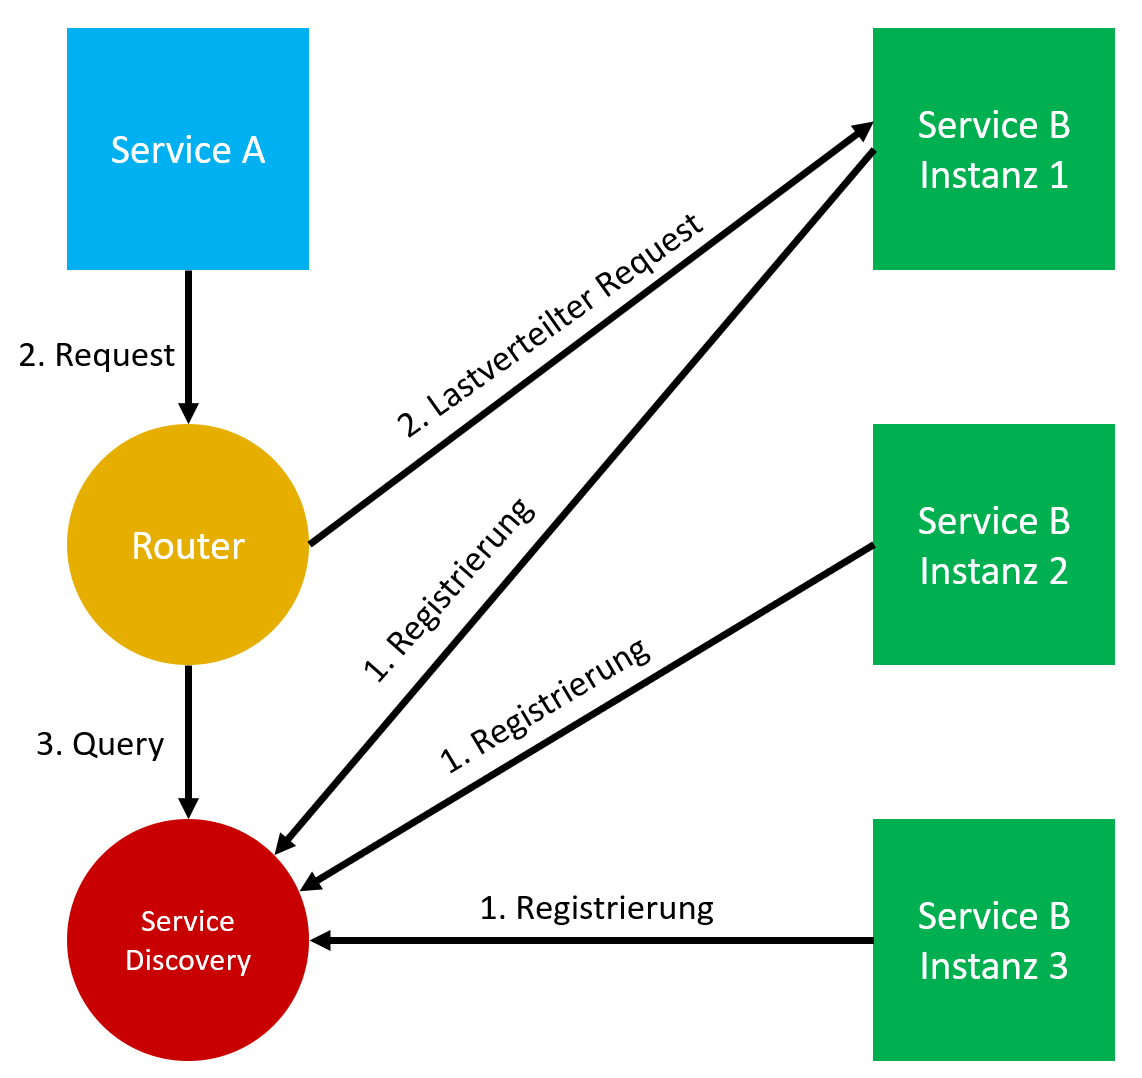
\includegraphics[width=0.65\linewidth]{images/service-discovery.png}
    \caption{Ablauf einer Anfrage mit der Service-Discovery - in Anlehnung an \cite{MichaelSchwab.2019}}
    \label{fig:service_discovery}
\end{figure}

\subsubsection*{Asynchrone Kommunikation}

Anders als bei der synchronen Kommunikation wird bei der asynchronen Kommunikation nicht auf jede Anfrage eine Antwort erwartet. Kern einer asynchronen Kommunikation ist ein zentraler Nachrichtenkanal, auf dem Nachrichten ausgetauscht werden. Ein Service schickt Nachrichten an solch einen Nachrichtenkanal, auch Message Broker genannt, und wenn ein andere Service an der Nachricht interessiert ist, kann er diese konsumieren. Eine Nachricht kann dabei auch von mehreren Services konsumiert werden.

Zu den bekanntesten Message Brokern zählen RabbitMQ und Apache Kafka. Während RabbitMQ leichtgewichtiger ist als Apache Kafka, hat letzteres mehr Features und weist eine größere Stabilität auf. Die Verantwortlichkeiten innerhalb des Systems werden bei der Verwendung eines Message Brokers umgedreht. Ein Service wird nun nicht mehr explizit von einem anderen Service aufgerufen, sondern schickt seine Nachrichten an den Message Broker, ohne zu wissen, wer dies Nachrichten konsumiert. Sender und Empfänger sind somit lose gekoppelt.

Zur Einteilung der Nachrichten werden in Message Brokern sogenannte Message Queues verwendet. Über eine Message Queue, welche einen bestimmten Topic besitzt, können Service dann entweder Nachrichten senden oder sich als Konsumenten an diesem Topic registrieren. In \autoref{fig:Message_Broker_Queue} ist die Funktionsweise von Apache Kafka abgebildet. Durch den Publish/Subscribe-Mechanismus kann Service A in diesem Beispiel sowohl Publisher von zwei Topics sein, als auch Konsument von einem Topic.

\begin{figure}[H]
    \centering
    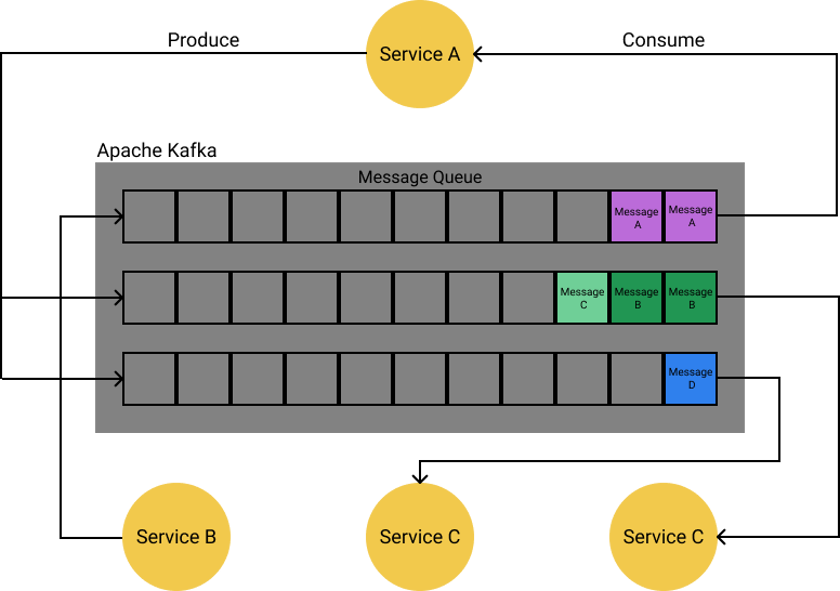
\includegraphics[width=0.65\linewidth]{images/apache-kafka.png}
    \caption{Funktion eines Message Brokers - \cite{MichaelSchwab.2019}}
    \label{fig:Message_Broker_Queue}
\end{figure}

Die Nachrichten werden in der Message Queue zwischengespeichert, bis die registrierten Konsumenten diese Nachrichten gelesen haben. Wenn ein Service sich an einer Message Queue registriert, können verschiedene Servicequalitäten für die Übertragung der Nachrichten angegeben werden. Folgende drei \glqq \gls{qos}\grqq{} können angegeben werden: \cite{ApacheSoftwareFoundation.2021}

\begin{description}
    \item[QoS 0 \glqq At most once\grqq{}:]\hfill \\
    Eine Nachricht wird genau einmal versendet. Nach dem Prinzip \glqq fire and forget\grqq{} wird keine Rückbestätigung erwartet. Verwendet wird diese Servicequalität meist für Nachrichten, welche mit einer hohen Frequenz versendet werden. So ist es für viele Sensoren in einer IoT-Umgebung nicht erforderlich, dass jeder gemessene Wert erfolgreich übermittelt werden muss.
    
    \item[QoS 1 \glqq At least once\grqq{}:]\hfill \\
    Es wird sichergestellt, dass eine Nachricht genau einmal beim Empfänger ankommt. Hierzu werden die Nachrichten beim Sender solange zwischengespeichert, bis vom Empfänger eine Bestätigung (PUBACK) empfangen wird. Wird über eine gewisse Zeitspanne keine Bestätigung empfangen, wird die Nachricht erneut versendet. Hierbei kann es vorkommen, dass ein Empfänger eine Nachricht mehrfach erhält. \cite{FlorianRaschbichler.2017}
    
    \item[QoS 2 \glqq Exactly once\grqq{}:]\hfill \\
    Eine Nachricht wird genau einmal zugesendet. Hierbei wird ein 4-Wege-Handshake zwischen Sender und Empfänger verwendet. Durch diesen Ablauf ist eine sichere Übertragung der Nachricht gewährleistet. Durch den großen Overhead ist jedoch diese Servicequalität die langsamste Übertragungsmöglichkeit.

\end{description}

\subsection{Microservice - Antipattern\label{subsec2.2.2:Unterunterpunkt-2}}

Um die Vorteile einer Microservice-Architektur im Bezug zur losen Kopplung und der damit eingehenden Unabhängigkeit der Microservices bezüglich Wartbarkeit und Erweiterbarkeit zu gewährleisten, ist es von Nöten die möglichen Antipattern einer Microservice-Architektur zu kennen. Mit hilfe von Antipattern können nach Roth und Hafner \cite{StephanRoth.2019} wiederkehrende Fehler bei der Softwareentwicklung identifiziert und in generalisierter Form dokumentiert werden. So können Antipattern dabei helfen häufig auftretende Fehler im vornherein zu vermeiden.

In einer Studie von Tighilt et al. \cite{Tighilt.072020} wurden 27 Paper und 67 Open-Source Anwendungen, welche alle Bezug zur Microservice-Architektur haben, untersucht. Die Ergebnisse der Studie \cite{Tighilt.072020} ergeben eine Sammlung von häufig aufgetretenen Antipatterns, welche durch Tighilt et al. in vier Kategorien unterteilt wurden. Folgend werden aus jeder Kategorie zwei Antipattern näher erläutert.

\subsubsection*{Design Antipattern}

In diese Kategorie gehören Antipattern, welche bereits in der architektonischen Entwurfsphase einer Microservice-Architektur zu Fehlern führen. Beispiele sind hierfür das \glqq Falscher Schnitt\grqq{}-Antipattern und das \glqq Zyklische Abhängigkeiten\grqq{}-Antipattern.

\begin{description}
    \item[Wrong Cut:]\hfill \\
    Beim \glqq Falscher Schnitt\grqq{}-Antipattern, wird die Aufteilung des Gesamtsystems in unterschiedliche Microservices nicht nach Geschäftsfunktionen, sondern nach technischen Aspekten durchgeführt. Ähnlich wie bei einer monolithischen 3-Schichten-Architektur übernehmen dann ein Teil der Microservices die Präsentationsschicht, andere Microservices wiederum bedienen die Geschäftsschicht und die anderen bedienen die Datenzugriffsschicht. Durch dieses Vorgehen verliert die Architekturen die lose Kopplung zwischen den Microservices und die Modularität geht verloren. Auch müssen bei einer Änderung einer Geschäftslogik mehrere Microservice abgeändert werden, was zu einem Mehraufwand führt.

    Verhindert werden kann dieses Antipattern indem man die Trennung des Gesamtsystems anhand der Geschäftsfunktionen durchführt. Jedes Microservices sollte von einem Team implementiert und gewartet werden können. Die Abhängigkeiten zu anderen Microservices sollte so gering, wie möglich ausfallen, um eine lose Kopplung und die Modularität der Architektur zu gewährleisten.
    
    \item[Zyklische Abhängigkeiten:]\hfill \\
    Ein weiterer Fehler ist die Missachtung der losen Kopplung, indem man mit zyklischen Abhängigkeiten eine zu große Abhängigkeit mit anderen Microservices verursacht. Bei sowohl der Implementierung als auch der Wartung solcher Microservices sind die abhängigen Microservices auch zu berücksichtigen. Dies erhöht die Komplexität und die Wahrscheinlichkeit, dass Fehler auftreten.

    Eine zyklische Abhängigkeit zwischen solchen Microservices kann verhindert werden, indem man stark voneinander abhängige Microservices in einen gemeinsamen Microservice zusammenfasst. 

\end{description}

\subsubsection*{Implementation Antipattern}

Implementation Antipattern entstehen aus der Art und Weise, wie Microservices implementiert werden. Beispiele sind hierfür das \glqq Gemeinsame Bibliotheken\grqq{}-Antipattern und das \glqq Festcodierte Endpunkte\grqq{}-Antipattern.

\begin{description}
    \item[Gemeinsame Bibliotheken:]\hfill \\
    Bei der Verwendung von gemeinsam benutzen Bibliotheken entstehen starke Abhängigkeiten und die Bibliotheken stellen einen sogenannten \glqq Single point of failure\grqq{} dar.

    Um dieses Problem zu umgehen, kann man jedem Microservice seine eigene Bibliothek zur Verfügung stellen. Dieser Ansatz wiederum führt zu einer Komplexität bei der Wartbarkeit der Microservice. Ein weitere Ansatz wäre es die Bibliotheken durch einen Bibliothek-Service zu abstrahieren. Die Microservices bleiben lose gekoppelt und die Komplexität bei der Wartung bleibt Überschaubar.
    
    \item[Festcodierte Endpunkte:]\hfill \\
    Bei der synchronen Kommunikation zwischen Microservices werden in der Regel Anfragen über REST APIs gestellt. Hierfür müssen die IP-Adresse und der Port des anderen Microservices bekannt sein. Ein Ansatz für schnelle Laufzeiten und eine schnelle Implementierung ist es, die Endpunkte fest im Quellcode zu hinterlegen. Jener Ansatz ist jedoch bei einer größeren Anzahl von Microservices nicht mehr wartbar. Sobald sich ein Endpunkt eines Microservice ändert, müssen alle abhängigen Microservices geändert und neu deployed werden.

    Abhilfe bringt die Einführung einer Service-Discovery (siehe \autoref{service_discovery}).

\end{description}

\subsubsection*{Deployment Antipattern}

Auch in der Bereitstellungsphase einer Microservice-Architektur können Fehler auftreten. Jene Antipattern werden Deployment Antipattern genannt. Beispiele sind hierfür das \glqq Manuelle Konfiguration\grqq{}-Antipattern und das \glqq Zeitüberschreitungen\grqq{}-Antipattern.

\begin{description}
    \item[Manuelle Konfiguration:]\hfill \\
    In einer Microservice-Architektur müssen aufgrund der Verteilung der Microservices auf unterschiedlichen Rechner verschiedene Konfigurationen durchgeführt werden. Eine manuelle Konfiguration von jedem Microservice führt zu unzähligen Konfigurationsdateien und Abhängigkeiten zu Umgebungsvariablen. Mit wachsender Anzahl von Microservices führt die manuelle Konfiguration zu einer ansteigenden Komplexität bei der Wartung der Konfigurationen.

    Vermieden werden kann das Antipattern durch die Einführung eines Konfigurations-Servers. Durch geeignete Konfigurationsmanagement-Tools können sämtliche Konfiguration zentral verwaltet werden.
    
    \item[Zeitüberschreitungen:]\hfill \\
    In einer verteilten Microservice-Architektur kann es vorkommen, dass einzelne Service ausfallen und nicht mehr zur Verfügung stehen. Hat nun ein anderer Microservice eine Anfrage über eine REST API gestellt, kann es vorkommen, dass unter Umständen gar keine Antwort kommt. Hierfür kann der Entwickler Timeouts festlegen, nach welchen einem anfragenden Service mitgeteilt wird, dass ein anderer Service nicht erreichbar ist. Den richtigen Wert für solch einen Timeout zu wählen, hängt von der Art des Service ab. Ein zu kurzer Timeout kann dazu führen, dass langsame Service frühzeitig beendet werden und bei einer zu langen Wahl des Timeouts kann es vorkommen, dass der Endnutzer zu lange warten muss, bis ihm signalisiert wird, dass der gewünschte Service nicht verfügbar ist.

    Um dem entgegen zu wirken verwendet man in einer Microservice-Architektur üblicherweise einen Circuit Breaker. Ein Circuit Breaker überwacht hierbei alle Instanzen einzelner Microservices und stellt fest, ob einzelne Timeouts bei der Kommunikation mit der jeweiligen Instanz überschritten wurden. Da solch ein Circuit Breaker als Proxy für alle Kommunikationskanäle verwendet wird, werden alle Anfragen an einen ausgefallenen Service mit einer Fehlermeldung beantwortet. Die Anfragen werden solange durch den Circuit Breaker blockiert, bis der ausgefallene Service wieder zur Verfügung steht. Auch der Timeout des Circuit Breaker muss vom Entwickler festgelegt werden. Jedoch liegt der Vorteil beim Blockieren der Anfragen an einen ausgefallenen Service, um so die Last von diesem zu nehmen.

\end{description}

\subsubsection*{Monitoring Antipattern}

Zu dem Betrieb einer Microservice-Architektur gehört auch die Überwachung der Änderungen im System. Hierbei kann es auch zu häufig auftretenden Antipattern kommen. Beispiele sind hierfür das \glqq Kein Gesundheitscheck\grqq{}-Antipattern und das \glqq Lokale Protokollierung\grqq{}-Antipattern.

\begin{description}
    \item[Kein Gesundheitscheck:]\hfill \\
    In der Natur der Microservices kann es vorkommen, dass einige Services über gewisse Zeitspannen nicht erreichbar sind. Um ein kompletten Systemausfall zu vermeiden, dienen Mechanismen, wie der Circuit Breaker dazu die anfragenden Service, nach dem überschreiten von Timeouts, zu benachrichtigen.

    Mit der Integration von Gesundheitschecks können solche Ausfälle von einzelnen Services im Vorraus erkannt und abhängige Microservices darüber informiert werden, dass das Senden von Anfragen zu unterlassen ist. Für solche Gesundheitschecks bietet es sich an API-Endpoints anzubieten, welche periodisch abgefragt werden können.
    
    \item[Lokale Protokollierung:]\hfill \\
    Um eine spätere Fehlerdiagnose zu ermöglichen, speichern Microservices einige Informationen über Änderungen in Log-Dateien. Ein häufiger Fehler ist, dass solch eine Protokollierung lokal in den Datenbanken der einzelnen Microservices gespeichert werden. Die Herausforderung liegt nun bei der Analyse und Abfrage von Logs aus verschiedenen Microservices.

    Mit einem verteilten Logging-Mechanismus können die Logs der unterschiedlichen Microservices in einem zentralen Speicherort gespeichert werden. Durch eine einheitliche Formatierung der Log-Einträge kann auch deren Abfrage und Analyse vereinfacht werden.

\end{description}

Auch bei der Integration einer Search Engine, in solch eine Microservice-Architektur, gilt es die vorgestellten Antipattern zu beachten, um so monolithische Seiteneffekte zu vermeiden.